\documentclass[11pt, a4paper]{article} %tamaño mínimo de letra 11pto.
\usepackage{amssymb}
\usepackage{amsmath}
\usepackage{amsfonts}
\usepackage{tikz}
\usetikzlibrary{arrows.meta}
\usepackage{hyperref}
\usepackage{graphicx} 
\usepackage{subcaption}
\usepackage[spanish]{babel} %Español 
\usepackage[utf8]{inputenc} %Para poder poner tildes
\usepackage{vmargin} %Para modificar los márgenes
\setmargins{2.5cm}{1.5cm}{16.5cm}{23.42cm}{10pt}{1cm}{0pt}{2cm}
%margen izquierdo, superior, anchura del texto, altura del texto, altura de los encabezados, espacio entre el texto y los encabezados, altura del pie de página, espacio entre el texto y el pie de página

%% \addbibresource{referencias.bib}

\begin{document}
%%%%%%Portada%%%%%%%
\begin{titlepage}
\centering
{ \bfseries \Large UNIVERSIDAD COMPLUTENSE DE MADRID}
\vspace{0.5cm}

{\bfseries  \Large FACULTAD DE CIENCIAS FÍSICAS} 
\vspace{1cm}

{\large DEPARTAMENTO DE ARQUITECTURA DE COMPUTADORES Y AUTOMÁTICA}
\vspace{0.8cm}

%%%%Logo Complutense%%%%%
{
\includegraphics[width=0.35\textwidth]{logo.png}} %Para ajustar la portada a una sola página se puede reducir el tamaño del logo
\vspace{0.8cm}

{\bfseries \Large TRABAJO DE FIN DE GRADO}
\vspace{2cm}

{\Large Código de TFG:  ACA07 } \vspace{5mm}

{\Large Control de sistemas multiagente y sus aplicaciones}\vspace{5mm}

{\Large Control of multi-agent systems and their applications}\vspace{5mm}

{\Large Supervisor/es: Lía García Pérez y Juan Jiménez Castellanos hola}\vspace{20mm} 

{\bfseries \LARGE YanRu Wu Jin}\vspace{5mm} 

{\large Grado en Física}\vspace{5mm} 

{\large Curso acad\'emico 2023-2024}\vspace{5mm} 

{\large Convocatoria XXXX}\vspace{5mm} 

\end{titlepage}
\newpage

{\bfseries \large Control de sistemas multiagente y sus aplicaciones }\vspace{10mm} 

{\bfseries \large Resumen:} \vspace{5mm}

Esto es una prueba para probar el formato del Resumen. Esto es una prueba para probar el formato del ResumenEsto es una prueba para probar el formato del ResumenEsto es una prueba para probar el formato del ResumenEsto es una prueba para probar el formato del ResumenEsto es una prueba para probar el formato del ResumenEsto es una prueba para probar el formato del ResumenEsto es una prueba para probar el formato del ResumenEsto es una prueba para probar el formato del ResumenEsto es una prueba para probar el formato del ResumenEsto es una prueba para probar el formato del ResumenEsto es una prueba para probar el formato del ResumenEsto es una prueba para probar el formato del ResumenEsto es una prueba para probar el formato del ResumenEsto es una prueba para probar el formato del Resumen.
\vspace{1cm}

{\bfseries \large Abstract: }\vspace{5mm} 

This is a test to prove the abstract's layout.This is a test to prove the abstract's layout.This is a test to prove the abstract's layout.This is a test to prove the abstract's layout.This is a test to prove the abstract's layout.This is a test to prove the abstract's layout.This is a test to prove the abstract's layout.This is a test to prove the abstract's layout.This is a test to prove the abstract's layout.This is a test to prove the abstract's layout.This is a test to prove the abstract's layout.This is a test to prove the abstract's layout.This is a test to prove the abstract's layout.This is a test to prove the abstract's layout.This is a test to prove the abstract's layout.This is a test to prove the abstract's layout.This is a test to prove the abstract's layout.This is a test to prove the abstract's layout.This is a test to prove the abstract's layout.
\vspace{1cm}

%%Comentar estas notas para que no salgan en la memoria
{\Large\textbf{Nota: el título extendido (si procede), el resumen y el abstract deben estar en una misma página y su extensión no debe superar una página. Tamaño mínimo 11pto.}}
\vspace{1cm}

{\Large\textbf{Extensión máxima 20 páginas sin contar portada ni resumen (sí se incluye índice, introducción, conclusiones y bibliografía}}
\newpage

\tableofcontents
\pagebreak

\section{Introducción}
Hoy en día el campo del control de sistemas se ha convertido en una de las disciplinas fundamentales y esenciales de la ingeniería y de la ciencia aplicada. Ejemplos como el sector aeronáutico, sistemas de transporte y de comunicaciones; todos requieren de un sistema de control para su correcto funcionamiento.\\

Dentro del control de sistemas, el control de enjambres es uno de los campos más fascinantes. Este se inspira en, como indica su nombre, los enjambres que se encuentran en la naturaleza \cite{TAN201318}, los cuales tienen una dinámica única capaz de controlar un grupo de agentes autónomos para que actúen como una única entidad coherente con unas instrucciones simples y locales seguidas por cada individuo. Algunos ejemplos podrían ser las bandadas de aves, bancos de peces o los enjambres de abejas.

\subsection{Objetivos}

Este trabajo se enfocará en construir un algoritmo capaz de guiar a un determinado número de agentes hacia una formación nominal y aplicar diferentes transformaciones afines a la formación, usando un enfoque \textit{leaderless}, es decir, sin un líder de formación. Basándose en un sistema de control de tensiones, se construirá una matriz Laplaciana que contendrá los pesos adecuados asociados a las conexiones entre los diferentes agentes. La dinámica del sistema vendrá dada entonces por esta matriz, alcanzando el sistema una configuración de consenso. Además,  se aplicaran transformaciones afines (ver Sección \ref{transform}) a la formación, modificando la matriz Laplaciana con los parámetros de la transformación. Por último, se explorarán las potenciales aplicaciones de este tipo de sistemas en el mundo actual, desde uso militar hasta en la medicina \cite{gold17283}.

\section{Definición del sistema}
\subsection{Notación }
Contamos con un número $n \in \mathbb{N}$ de agentes móviles.Se denota $||x||$ como la norma euclideana del vector $x \in \mathbb{R}^p$, $p\in\mathbb{N}$ , y dado un conjunto $\mathcal{X}$, su cardinalidad será definida como $|\mathcal{X}|$ . El vector columna formado por todo unos se representará por $\boldsymbol{1}_n$ y, dada una matriz $A \in \mathbb{R}^{p\times q}$, $p, q\in \mathbb{N}$, se define el operador $\overline{A}:= A\otimes I_m \in \mathbb{R}^{pm\times qm}$, donde $\otimes$ es el producto de Kronecker y $I_m \in \mathbb{R}^m$ es la matriz identidad. \\


Definiremos un grafo no dirigido como \cite{9682800} $\mathcal{G} = \{\mathcal{V},\mathcal{E}\}$, donde $\mathcal{V} = \{1,2,\dots,n\}$, $\mathcal{E} \subseteq (\mathcal{V}\times\mathcal{V})$, son conjuntos no vacíos de los nodos y pares de nodos sin ordenar (o aristas), respectivamente. Un grafo no dirigido es un grafo bidireccional donde las aristas no tienen una dirección de preferencia. 

El conjunto $\mathcal{N}_i$ contiene a los vecinos del nodo $i$, y está definido como $\mathcal{N}_i := \{j \in \mathcal{V}: (i,j)\in\mathcal{E}\}$, lo cual indica que los vecinos de $i$ son aquellos con los que está conectado por una arista de $\mathcal{E}$.

Sea $\omega_{ij}\in \mathbb{R}$ el peso asociado al nodo $(i,j) \in \mathcal{E}$, de tal modo que la matriz Laplaciana $L \in \mathbb{R}^{n\times n}$ de $G$ se define como:

\begin{equation}
l_{ij} :=
\begin{cases} 
\sum_{k \in \mathcal{N}_i} w_{ik} & \text{si } i = j, \\ 
-w_{ij} & \text{si } i \neq j \land j \in \mathcal{N}_i, \\ 
0 & \text{si } i \neq j \land j \notin \mathcal{N}_i.
\end{cases}
\end{equation}

Asumimos que el grafo es conexo, esto es \cite{GTMMN}, para cada par de nodos $(i,j)\in \mathcal{E}$, existe al menos un camino (secuencia de aristas consecutivas) que los conecta, por lo que $L\boldsymbol{1}_n = 0$. Ya que tratamos con un grafo no dirigido, para cada par de nodos vecinos escogeremos una dirección arbitraria para construir un conjunto ordenado de nodos, $\mathcal{Z}$, de tal forma que para un nodo arbitrario $\mathcal{Z}_k = (\mathcal{Z}_k^{head}, \mathcal{Z}_k^{tail},\, k \in \{1,\dots,\frac{|\mathcal{E}|}{2}\}$, donde el primer elemento será la \textit{cabeza} y el segundo, la \textit{cola}. Esto será útil para construir una matriz de incidencia $H\in\mathbb{R}^{|\mathcal{Z}|\times|\mathcal{V}|}$ que satisface también $H\boldsymbol{1}_n =0$:

\begin{equation}
H_{ik} :=
\begin{cases} 
+1 & \text{si } i = \mathcal{Z}_{k}^{\text{tail}}, \\ 
-1 & \text{si } i = \mathcal{Z}_{k}^{\text{head}}, \\ 
0 & \text{en otro caso}.
\end{cases}
\end{equation}

\subsubsection{Formación nominal}
Llamaremos \textit{configuración} del conjunto de nodos $n\in\mathcal{V}$ a sus coordenadas apiladas en el espacio Euclideo $p\in\mathbb{R}^{dn}$, $p = [p_1^T,\dots, p_n^T]^T$. Llamaremos estructura, \textit{framework}, a un grafo equipado con una configuración, de tal forma que $\mathcal{F}=(\mathcal{G}, p)$. La figura \ref{fig:framework} muestra un ejemplo de estructura.

A partir de la configuración definiremos la \textit{matriz de configuración}, $P\in\mathbb{R}^{n\times d}$ y la \textit{matriz de configuración aumentada} $\Bar{P}\in\mathbb{R}^{n\times (d+1)}$ como:

\begin{equation}
P(p) = 
\begin{bmatrix}
p_1^T \\
\vdots \\
p_n^T
\end{bmatrix},
\quad
\Bar{P}(p) = 
\begin{bmatrix}
p_1^T & 1 \\
\vdots & \vdots \\
p_n^T & 1
\end{bmatrix}
= \begin{bmatrix}
P(p), & \boldsymbol{1}_n
\end{bmatrix}
\end{equation}

Denotamos la formación nominal $p^*$ para el grupo de agentes como:
\begin{equation}
    p^* = (\boldsymbol{1}_n \otimes p_\text{c.m.}) + p^*_c
\end{equation}

De tal manera que $p_\text{c.m.}$ es la posición del centro de masas de la configuración y $p^*_c$ son las coordenadas de los nodos desde el centro de masas, que dará a la formación su apariencia. En este trabajo se simplificará esto imponiendo $p_\text{c.m.} = 0$. Además asumiremos que $p^*$ como genérica. Eso es \cite{7339680}, si todas las coordenadas $p_1,\dots p_n$ son algebraicamente independientes sobre los enteros, en otras palabras, no existe un polinomio no nulo con coeficientes enteros tal que $f(p_1^1,\dots,p_1^m,\dots,p_n^1,\dots,p_n^m)= 0$, donde $p_i^j$ es el $j\text{-ésimo}$ elemento del vector $p_i$.
\begin{figure}[h!]
    \centering
    \begin{tikzpicture}[scale=1]
    
    \coordinate (p1) at (-1, -1);
    \coordinate (p2) at (-1, 1);
    \coordinate (p3) at (1, -1);
    \coordinate (p4) at (1, 1);
    \coordinate (p5) at (2, 0);
    \coordinate (p6) at (-2, 0);
    
    \draw (p1) -- (p2);
    \draw (p1) -- (p3);
    \draw (p1) -- (p5);
    \draw (p1) -- (p6);
    \draw (p2) -- (p4);
    \draw (p2) -- (p5);
    \draw (p2) -- (p6);
    \draw (p3) -- (p4);
    \draw (p3) -- (p5);
    \draw (p3) -- (p6);
    \draw (p4) -- (p5);
    \draw (p4) -- (p6);
    
    \fill[red] (p1) circle (2pt) ;
    \node at (p1) [below left] {$1$};
    \fill[red] (p2) circle (2pt) ;
    \node at (p2) [above left] {$2$};
    \fill[red] (p3) circle (2pt) ;
    \node at (p3) [below right] {$3$};
    \fill[red] (p4) circle (2pt) ;
    \node at (p4) [above right] {$4$};
    \fill[red] (p5) circle (2pt) ;
    \node at (p5) [right] {$5$};
    \fill[red] (p6) circle (2pt) ;
    \node at (p6) [left] {$6$};
    
    \end{tikzpicture}
\caption{Ejemplo de \textit{framework}}
\label{fig:framework}
\end{figure}


\subsubsection{Obtención de pesos $\omega_{ij}$}
Considerando la dirección definida para la matriz de incidencia $H$, definimos $h_i\in\mathbb{R}^{|\mathcal{Z}|}$ como la $i$-ésima columna de $H$, y por tanto $H = [h_1,\dots,h_n]$, definiremos la matriz $E\in\mathbb{R}^{n(d+1)\times|\mathcal{Z}|}$:

\begin{equation}
E = 
\begin{bmatrix}
\Bar{P}^T(r) H^T \text{diag}(h_1) \\
\vdots \\
\Bar{P}^T(r) H^T \text{diag}(h_n)
\end{bmatrix}
\end{equation}

\subsection{Condición de estabilidad}
Para que una formación afín sea estabilizable sobre un grafo no dirigido \cite{7339680}, debe cumplirse la condición de que el grafo es genéricamente y universalmente rígido. 

La condición genérica se cumple al ser $p$ genérica.

Dos \textit{frameworks} $(\mathcal{G},p)$ en $\mathbb{R}^{m_1}$ y $(\mathcal{G},q)$ en $\mathbb{R}^{m_2}$ son equivalentes ($\equiv$) si las distancias entre pares de nodos se preservan con aristas (se mantiene la escala). Dos \textit{frameworks} serán congruentes ($\cong$ si $p$ y $q$ se pueden obtener el uno del otro por un movimiento rígido como traslación o rotación (se mantiene la forma).
Un \textit{framework} en $\mathbb{R}^m$ es universalmente rígido si para cualquier configuración $q$ en $\mathbb{R}^s$, $s\in\mathbb{N}$, $(\mathcal{G},p) \equiv (\mathcal{G}, q)$ implica $(\mathcal{G},p) \cong (\mathcal{G}, q)$.

Podemos realizar la prueba con el \textit{framework} de la figura \ref{fig:frameworknoestable}, el cual no es universalmente rígido ya que en $\mathbb{R}^3$, el triángulo $\triangle 345$ se puede “plegar” sobre la arista (3,4), incumpliendo la condición dada de rigidez universal. Con la ayuda de las simulaciones (figura \ref{fig:simulnoestable}) nos damos cuenta de que el agente 5 no se estabiliza con el resto. Añadiendo una arista más (fig \ref{fig:frameworkestable}), (1,5) o (2,5), se cumpliría con la condición de rigidez, por lo que el sistema sí sería estabilizable (figura \ref{fig:simulestable}).


\begin{figure}[h!]
        \centering
        \begin{subfigure}[t]{0.45\textwidth}
            \centering
            \begin{tikzpicture}[scale=1]
            \coordinate (p1) at (-1, 1);
            \coordinate (p2) at (-1, -1);
            \coordinate (p3) at (1, -1);
            \coordinate (p4) at (1, 1);
            \coordinate (p5) at (2, 0);
            
            \draw (p1) -- (p2);
            \draw (p1) -- (p3);
            \draw (p2) -- (p4);
            \draw (p3) -- (p4);
            \draw (p3) -- (p5);
            \draw (p4) -- (p5);
            \draw (p1) -- (p4);
            \draw (p2) -- (p3);
            \draw [blue, dashed ,-Triangle] (p5) --  (1.5,0);
            
            \fill[red] (p2) circle (2pt) ;
            \node at (p2) [below left] {$2$};
            \fill[red] (p1) circle (2pt) ;
            \node at (p1) [above left] {$1$};
            \fill[red] (p3) circle (2pt) ;
            \node at (p3) [below right] {$3$};
            \fill[red] (p4) circle (2pt) ;
            \node at (p4) [above right] {$4$};
            \fill[red] (p5) circle (2pt) ;
            \node at (p5) [right] {$5$};

            \end{tikzpicture}
            
            \caption{\textit{Framework} no universalmente rígido}
            \label{fig:frameworknoestable}
        \end{subfigure}
        \hspace{0.5cm}
        \begin{subfigure}[t]{0.45\textwidth}
            \centering
            \begin{tikzpicture}[scale=1]
            \coordinate (p1) at (-1, 1);
            \coordinate (p2) at (-1, -1);
            \coordinate (p3) at (1, -1);
            \coordinate (p4) at (1, 1);
            \coordinate (p5) at (2, 0);
            
            \draw (p1) -- (p2);
            \draw (p1) -- (p3);
            \draw (p2) -- (p4);
            \draw (p3) -- (p4);
            \draw (p3) -- (p5);
            \draw (p4) -- (p5);
            \draw (p1) -- (p4);
            \draw (p2) -- (p3);
            \draw (p1) -- (p5);
            
            \fill[red] (p2) circle (2pt) ;
            \node at (p2) [below left] {$2$};
            \fill[red] (p1) circle (2pt) ;
            \node at (p1) [above left] {$1$};
            \fill[red] (p3) circle (2pt) ;
            \node at (p3) [below right] {$3$};
            \fill[red] (p4) circle (2pt) ;
            \node at (p4) [above right] {$4$};
            \fill[red] (p5) circle (2pt) ;
            \node at (p5) [right] {$5$};
            
            \end{tikzpicture}
            
            \caption{\textit{Framework} universalmente rígido}
            \label{fig:frameworkestable}
        \end{subfigure}
    \caption{\textit{Frameworks} y manipulación de rigidez}

        \centering
        \begin{subfigure}[t]{0.46\textwidth}
            \centering
            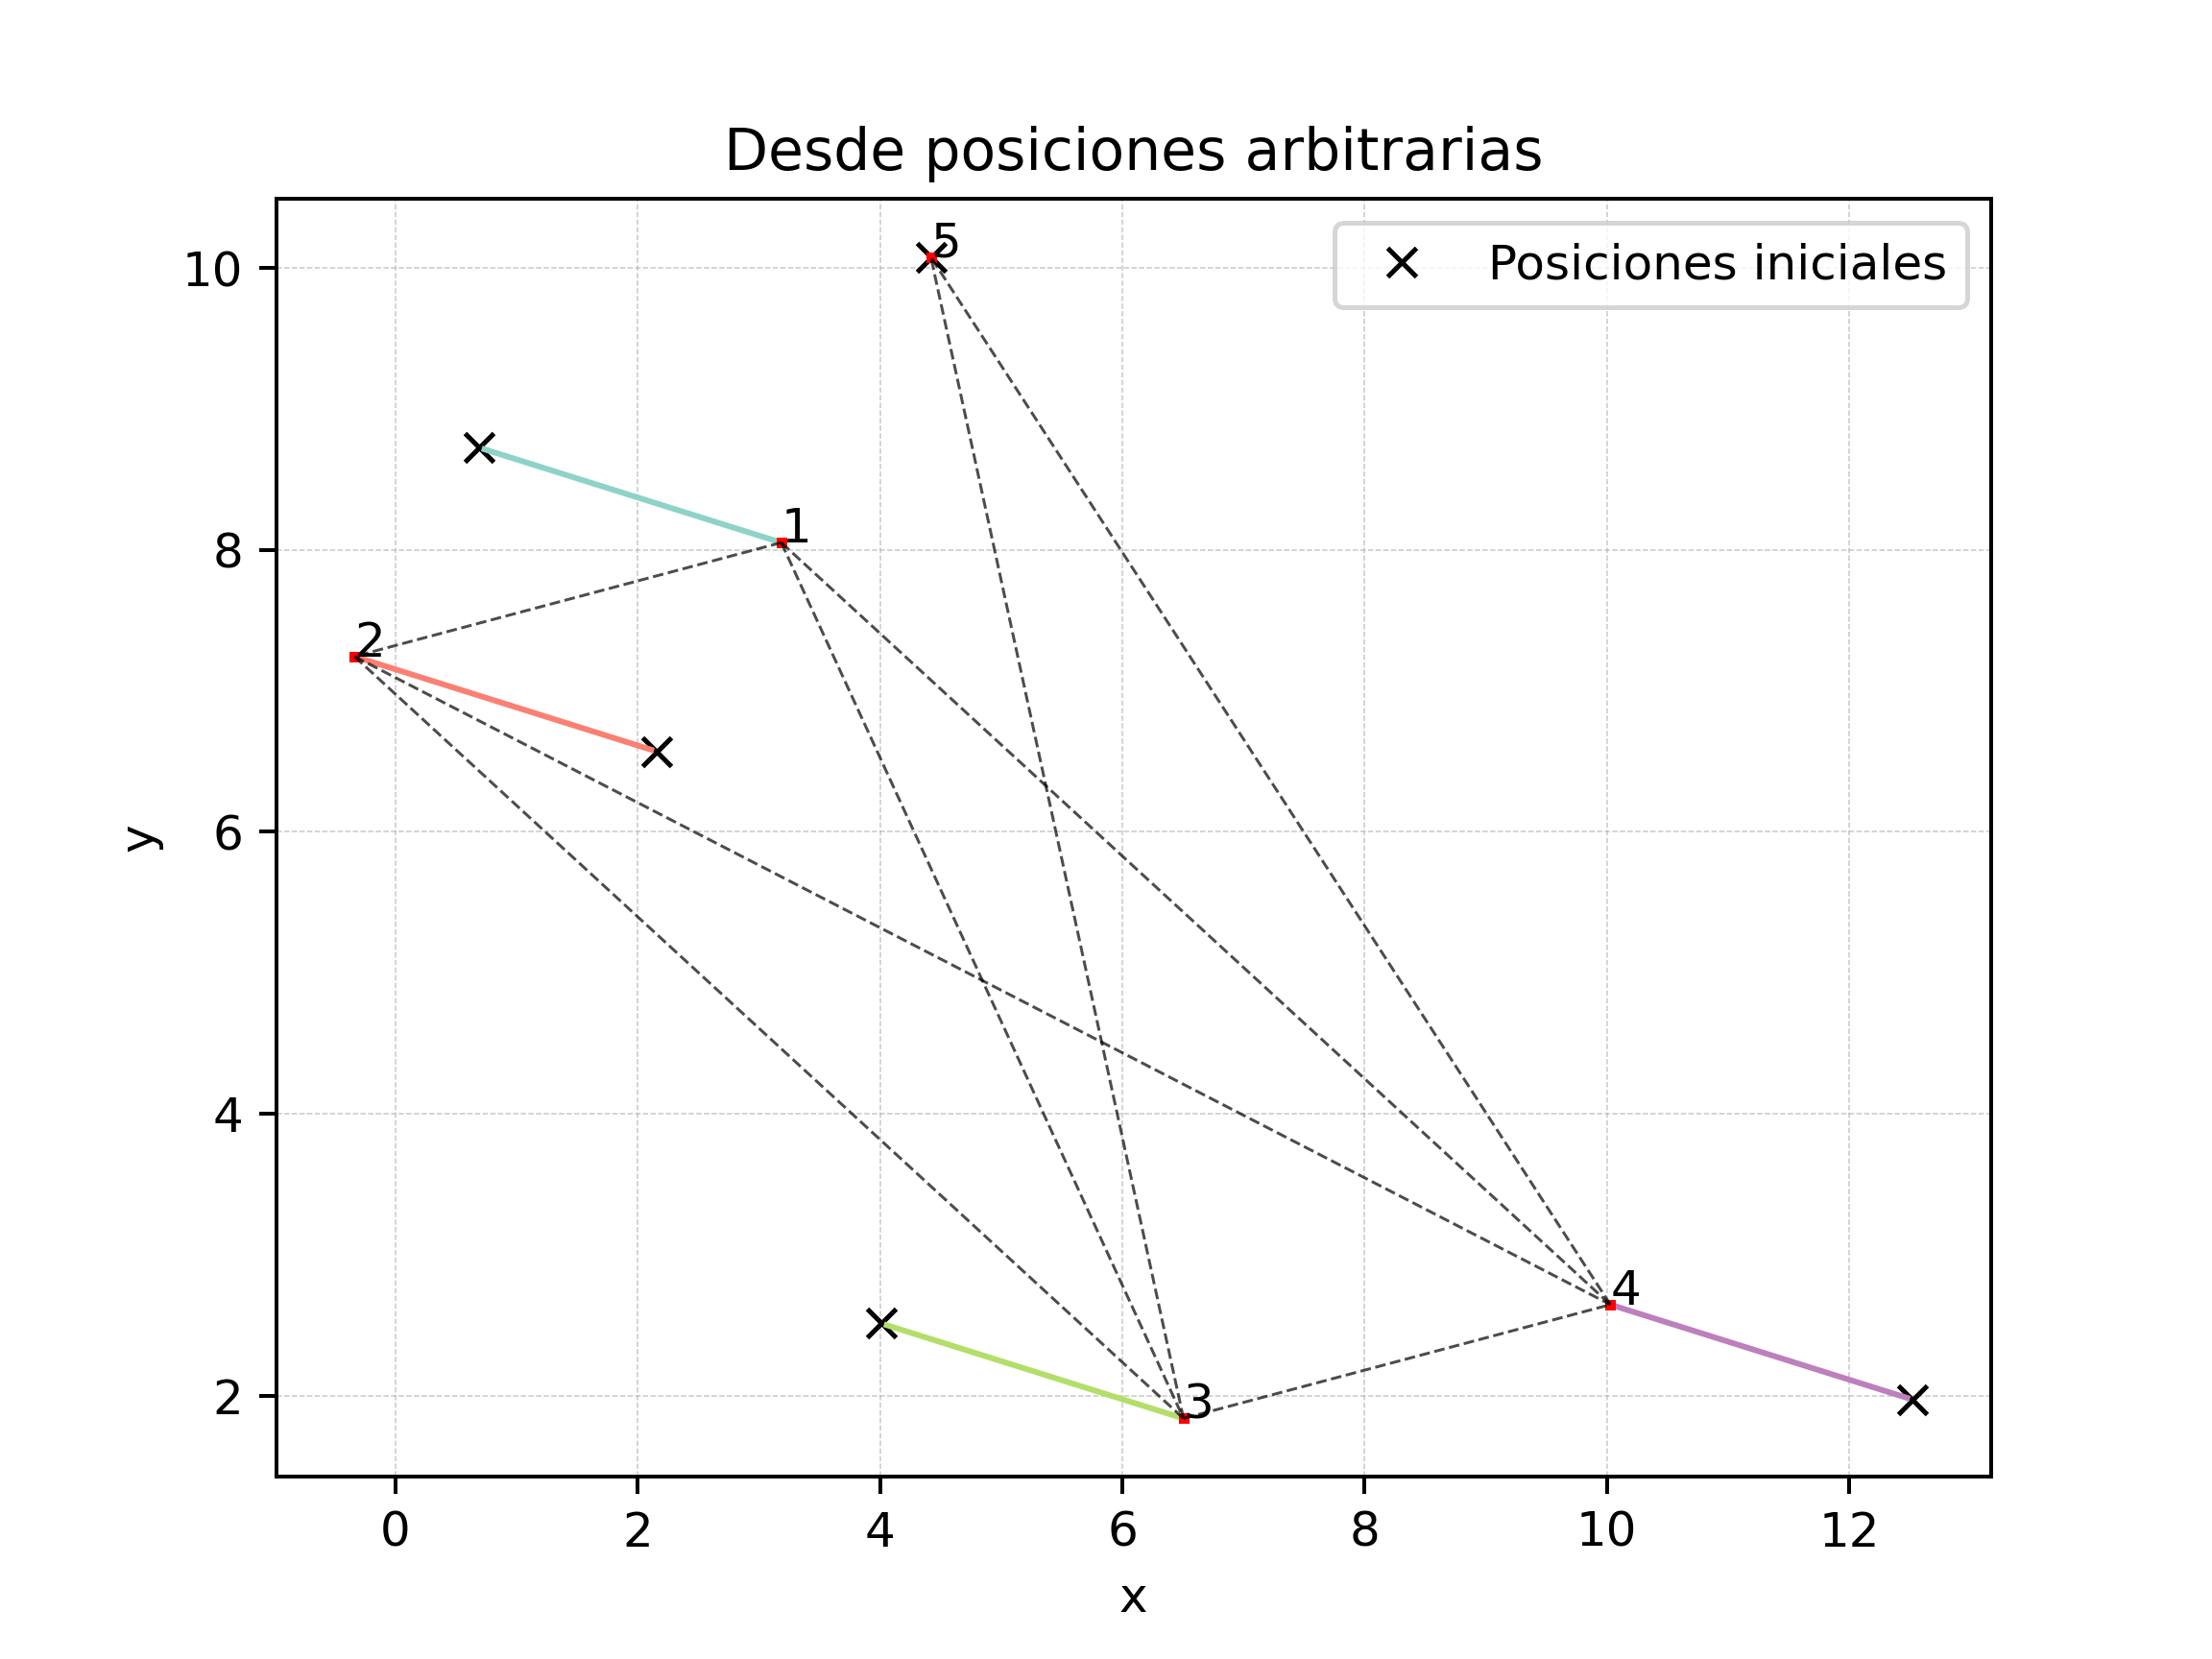
\includegraphics[width=\linewidth]{No estabilizable.png}
            \caption{Simulación con \textit{framework} no rígido.}
            \label{fig:simulnoestable}
        \end{subfigure}
        \hspace{0.5cm}
        \begin{subfigure}[t]{0.46\textwidth}
            \centering
            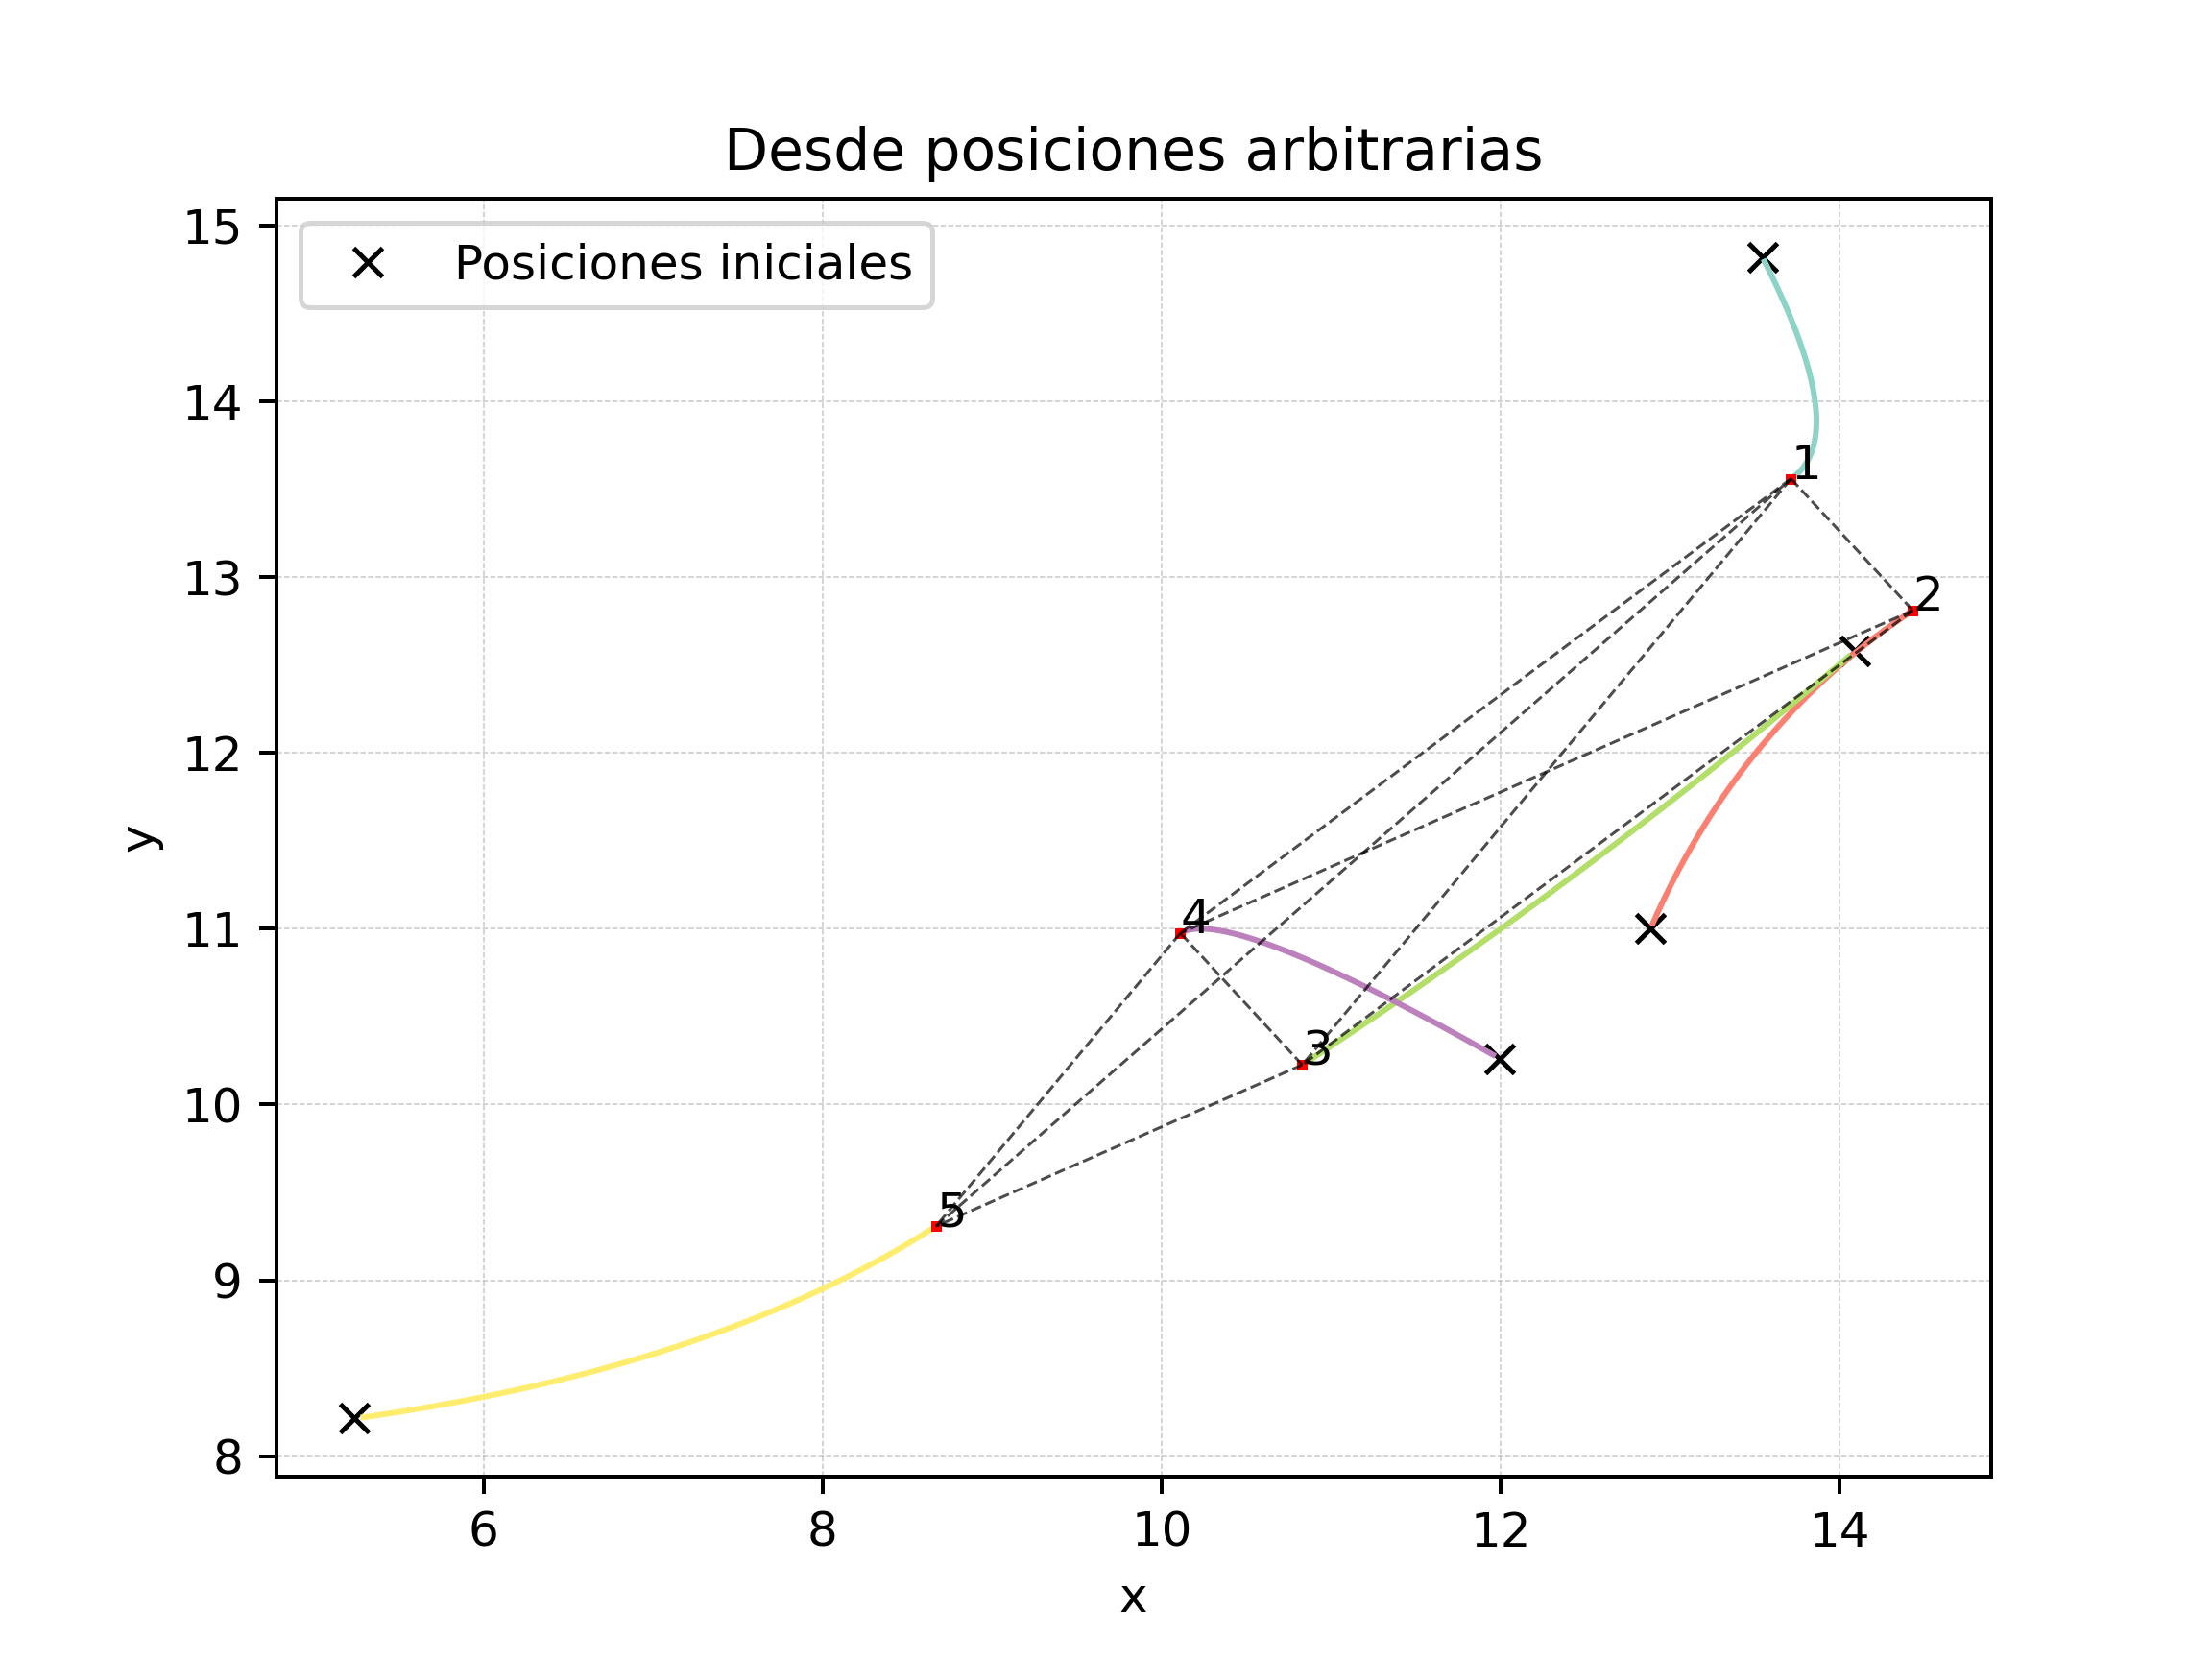
\includegraphics[width=\linewidth]{estabilizable.png}
            \caption{Simulación con \textit{framework} rígido}
            \label{fig:simulestable}
        \end{subfigure}
        \caption{Simulaciones según rigidez}
\end{figure}



\section{Parámetros de transformación} \label{transform}


\section{Resultados}

\begin{figure}
	\begin{subfigure}[t]{0.46\textwidth}
    	\centering
    	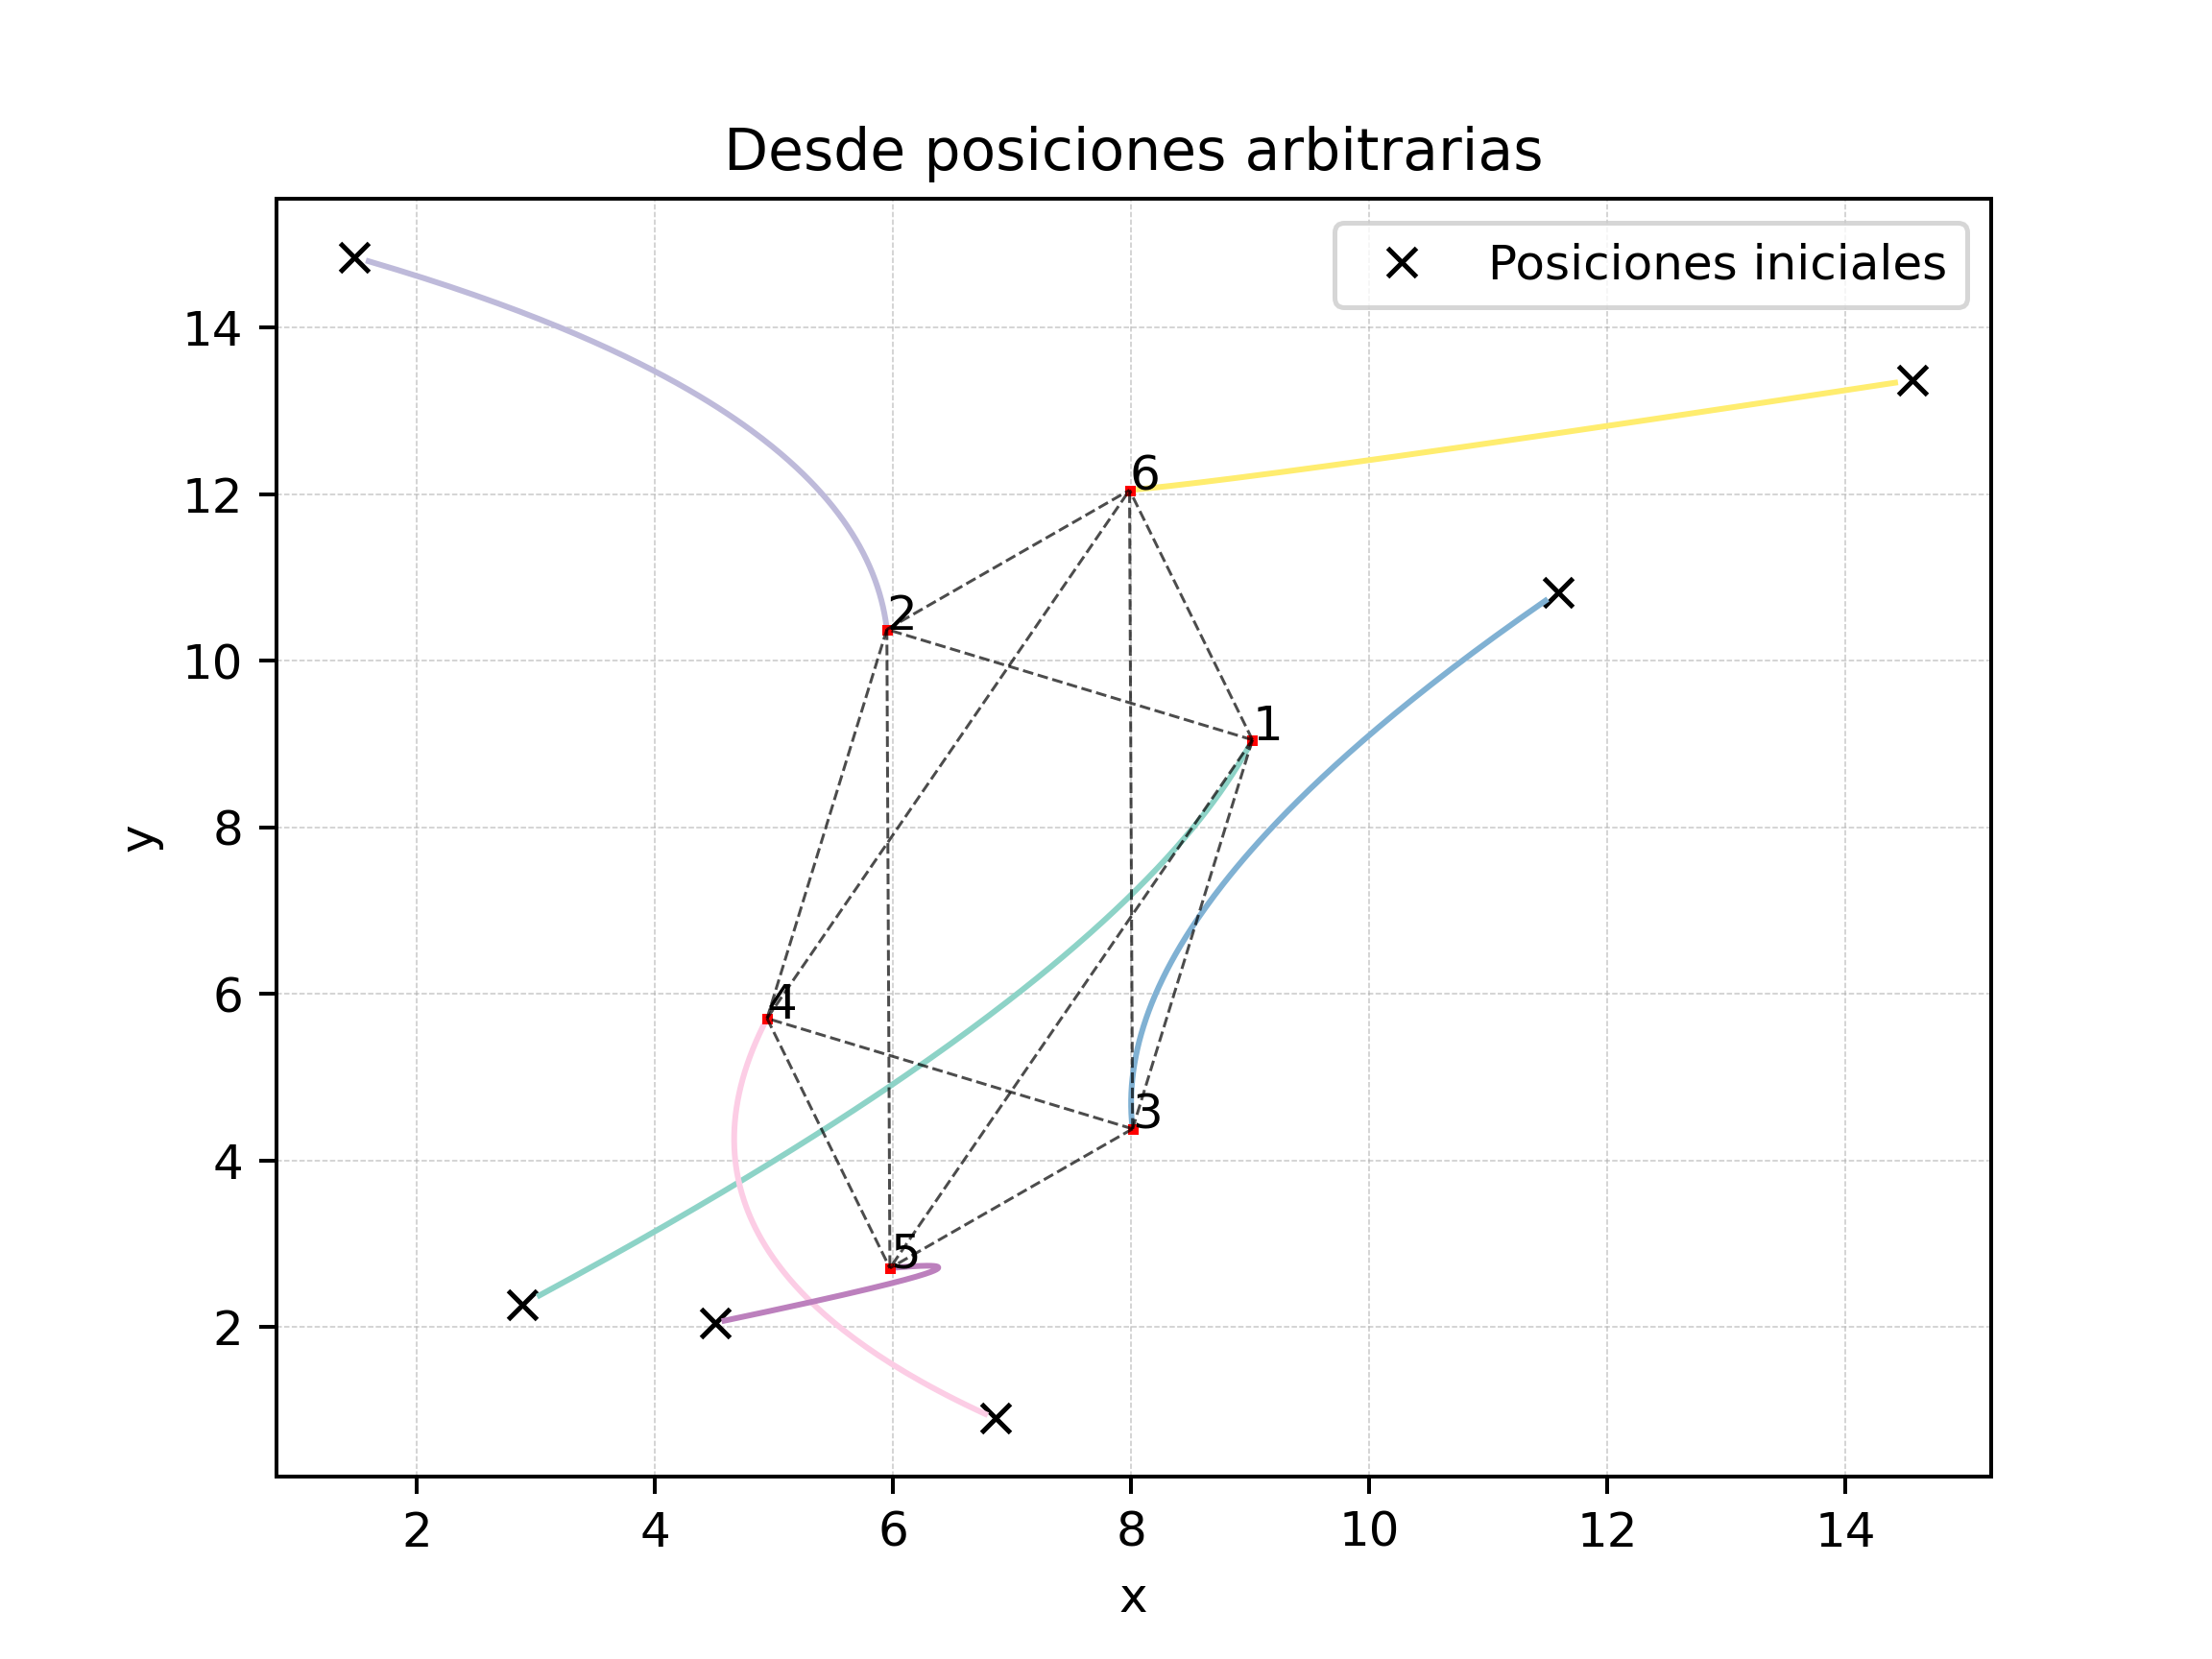
\includegraphics[width=\linewidth]{posiciones.arb2d.png}
    	\caption{Enter Caption}
    	\label{fig:2dcombi}
	\end{subfigure}
	\hspace{0.1cm}
	\begin{subfigure}[t]{0.46\textwidth}
    	\centering
    	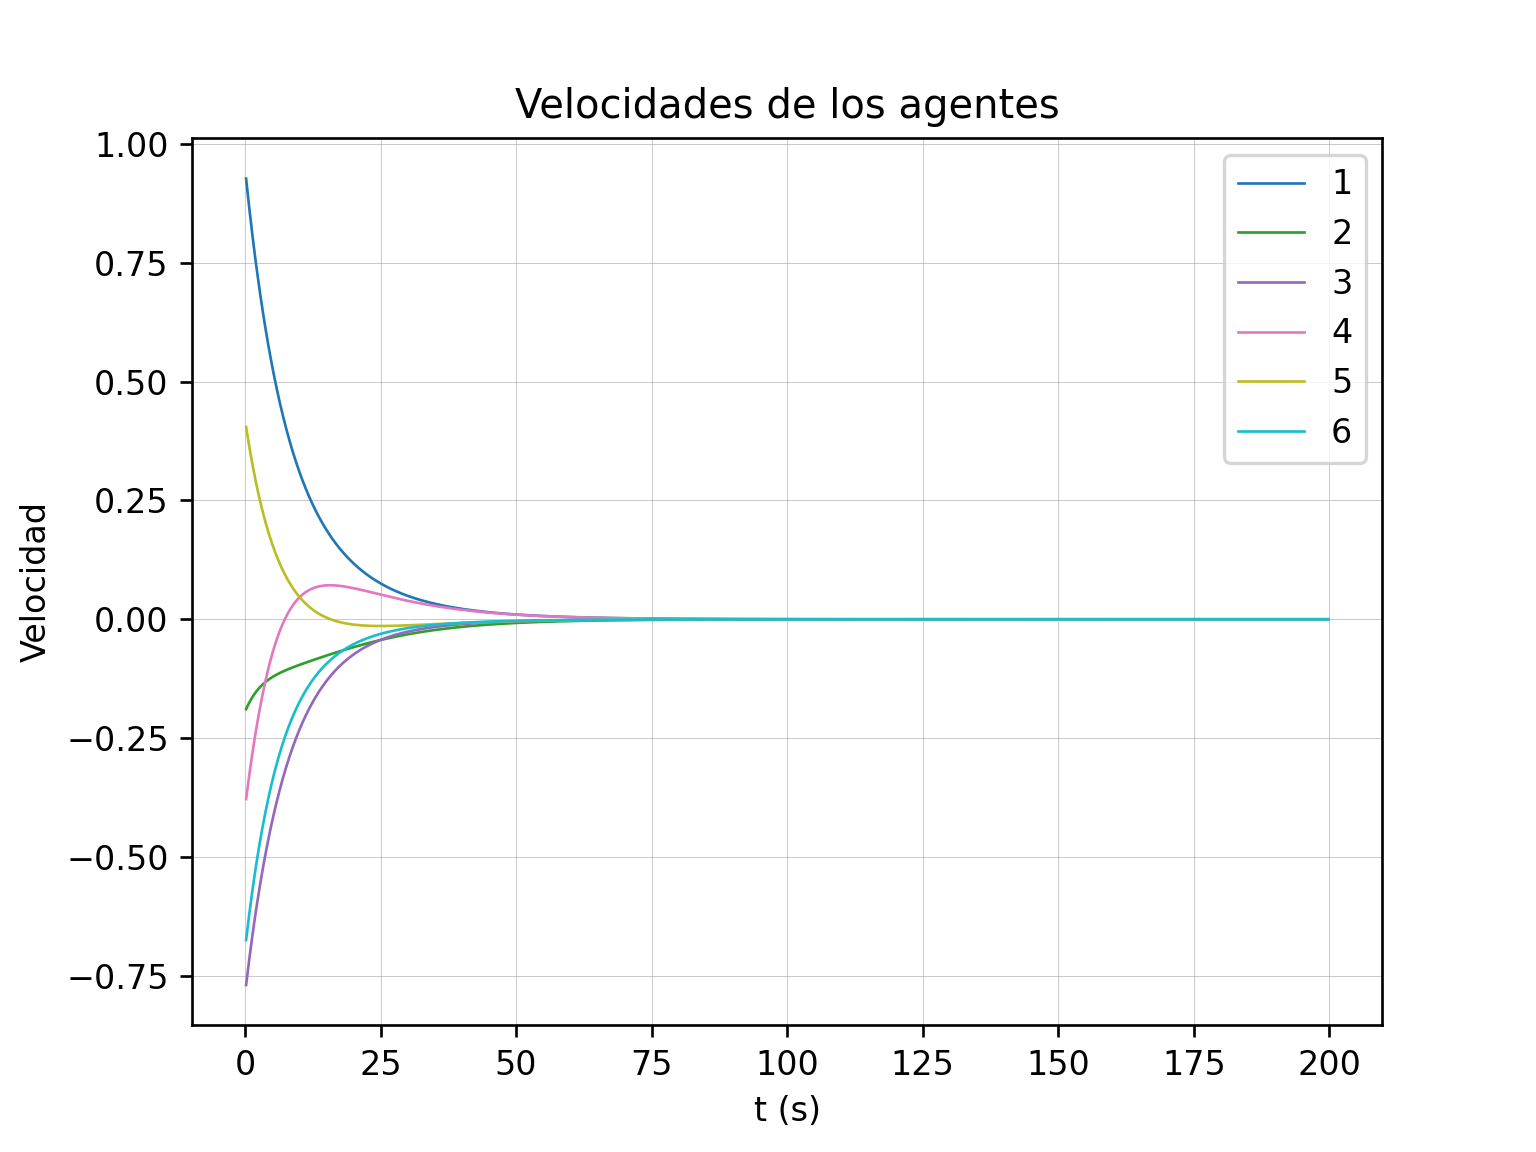
\includegraphics[width=\linewidth]{vels.2d.png}
    	\caption{Enter Caption}
    	\label{fig:3dcombi}
	\end{subfigure}
\end{figure}


\pagebreak
\bibliographystyle{plain}
\bibliography{referencias}
\end{document}
